\documentclass[twoside]{book}

% Packages required by doxygen
\usepackage{calc}
\usepackage{doxygen}
\usepackage{graphicx}
\usepackage[utf8]{inputenc}
\usepackage{makeidx}
\usepackage{multicol}
\usepackage{multirow}
\usepackage{textcomp}
\usepackage[table]{xcolor}

% Font selection
\usepackage[T1]{fontenc}
\usepackage{mathptmx}
\usepackage[scaled=.90]{helvet}
\usepackage{courier}
\usepackage{amssymb}
\usepackage{sectsty}
\renewcommand{\familydefault}{\sfdefault}
\allsectionsfont{%
  \fontseries{bc}\selectfont%
  \color{darkgray}%
}
\renewcommand{\DoxyLabelFont}{%
  \fontseries{bc}\selectfont%
  \color{darkgray}%
}

% Page & text layout
\usepackage{geometry}
\geometry{%
  a4paper,%
  top=2.5cm,%
  bottom=2.5cm,%
  left=2.5cm,%
  right=2.5cm%
}
\tolerance=750
\hfuzz=15pt
\hbadness=750
\setlength{\emergencystretch}{15pt}
\setlength{\parindent}{0cm}
\setlength{\parskip}{0.2cm}
\makeatletter
\renewcommand{\paragraph}{%
  \@startsection{paragraph}{4}{0ex}{-1.0ex}{1.0ex}{%
    \normalfont\normalsize\bfseries\SS@parafont%
  }%
}
\renewcommand{\subparagraph}{%
  \@startsection{subparagraph}{5}{0ex}{-1.0ex}{1.0ex}{%
    \normalfont\normalsize\bfseries\SS@subparafont%
  }%
}
\makeatother

% Headers & footers
\usepackage{fancyhdr}
\pagestyle{fancyplain}
\fancyhead[LE]{\fancyplain{}{\bfseries\thepage}}
\fancyhead[CE]{\fancyplain{}{}}
\fancyhead[RE]{\fancyplain{}{\bfseries\leftmark}}
\fancyhead[LO]{\fancyplain{}{\bfseries\rightmark}}
\fancyhead[CO]{\fancyplain{}{}}
\fancyhead[RO]{\fancyplain{}{\bfseries\thepage}}
\fancyfoot[LE]{\fancyplain{}{}}
\fancyfoot[CE]{\fancyplain{}{}}
\fancyfoot[RE]{\fancyplain{}{\bfseries\scriptsize Generated on Sat Mar 22 2014 18\-:24\-:56 for 3k Stabilizer client by Doxygen }}
\fancyfoot[LO]{\fancyplain{}{\bfseries\scriptsize Generated on Sat Mar 22 2014 18\-:24\-:56 for 3k Stabilizer client by Doxygen }}
\fancyfoot[CO]{\fancyplain{}{}}
\fancyfoot[RO]{\fancyplain{}{}}
\renewcommand{\footrulewidth}{0.4pt}
\renewcommand{\chaptermark}[1]{%
  \markboth{#1}{}%
}
\renewcommand{\sectionmark}[1]{%
  \markright{\thesection\ #1}%
}

% Indices & bibliography
\usepackage{natbib}
\usepackage[titles]{tocloft}
\setcounter{tocdepth}{3}
\setcounter{secnumdepth}{5}
\makeindex

% Hyperlinks (required, but should be loaded last)
\usepackage{ifpdf}
\ifpdf
  \usepackage[pdftex,pagebackref=true]{hyperref}
\else
  \usepackage[ps2pdf,pagebackref=true]{hyperref}
\fi
\hypersetup{%
  colorlinks=true,%
  linkcolor=blue,%
  citecolor=blue,%
  unicode%
}

% Custom commands
\newcommand{\clearemptydoublepage}{%
  \newpage{\pagestyle{empty}\cleardoublepage}%
}


%===== C O N T E N T S =====

\begin{document}

% Titlepage & ToC
\hypersetup{pageanchor=false}
\pagenumbering{roman}
\begin{titlepage}
\vspace*{7cm}
\begin{center}%
{\Large 3k Stabilizer client }\\
\vspace*{1cm}
{\large Generated by Doxygen 1.8.6}\\
\vspace*{0.5cm}
{\small Sat Mar 22 2014 18:24:56}\\
\end{center}
\end{titlepage}
\clearemptydoublepage
\tableofcontents
\clearemptydoublepage
\pagenumbering{arabic}
\hypersetup{pageanchor=true}

%--- Begin generated contents ---
\chapter{Hierarchical Index}
\section{Class Hierarchy}
This inheritance list is sorted roughly, but not completely, alphabetically\-:\begin{DoxyCompactList}
\item Q\-Dialog\begin{DoxyCompactList}
\item \contentsline{section}{Dialog\-Menu}{\pageref{class_dialog_menu}}{}
\end{DoxyCompactList}
\item Q\-Main\-Window\begin{DoxyCompactList}
\item \contentsline{section}{Main\-Window}{\pageref{class_main_window}}{}
\end{DoxyCompactList}
\item Q\-Thread\begin{DoxyCompactList}
\item \contentsline{section}{Thread\-Receiving}{\pageref{class_thread_receiving}}{}
\item \contentsline{section}{Thread\-Sending}{\pageref{class_thread_sending}}{}
\end{DoxyCompactList}
\item \contentsline{section}{User\-Data}{\pageref{class_user_data}}{}
\end{DoxyCompactList}

\chapter{Class Index}
\section{Class List}
Here are the classes, structs, unions and interfaces with brief descriptions\-:\begin{DoxyCompactList}
\item\contentsline{section}{\hyperlink{class_dialog_menu}{Dialog\-Menu} \\*The menu window where the user can parametrize its stabilizer inherits from Q\-Dialog }{\pageref{class_dialog_menu}}{}
\item\contentsline{section}{\hyperlink{class_main_window}{Main\-Window} \\*Main window of the application, implements view and user actions inherits from Q\-Main\-Window }{\pageref{class_main_window}}{}
\item\contentsline{section}{\hyperlink{class_thread_receiving}{Thread\-Receiving} \\*Thread establishing connections and receives data from the server }{\pageref{class_thread_receiving}}{}
\item\contentsline{section}{\hyperlink{class_thread_sending}{Thread\-Sending} \\*Thread establishing connection with server and sends data to the server inherits from Q\-Thread }{\pageref{class_thread_sending}}{}
\item\contentsline{section}{\hyperlink{class_user_data}{User\-Data} \\*User data(the offset he has chosen for his stabilizer) }{\pageref{class_user_data}}{}
\end{DoxyCompactList}

\chapter{Class Documentation}
\hypertarget{class_dialog_menu}{\section{Dialog\-Menu Class Reference}
\label{class_dialog_menu}\index{Dialog\-Menu@{Dialog\-Menu}}
}


The menu window where the user can parametrize its stabilizer inherits from Q\-Dialog.  




{\ttfamily \#include $<$dialogmenu.\-h$>$}

Inheritance diagram for Dialog\-Menu\-:\begin{figure}[H]
\begin{center}
\leavevmode
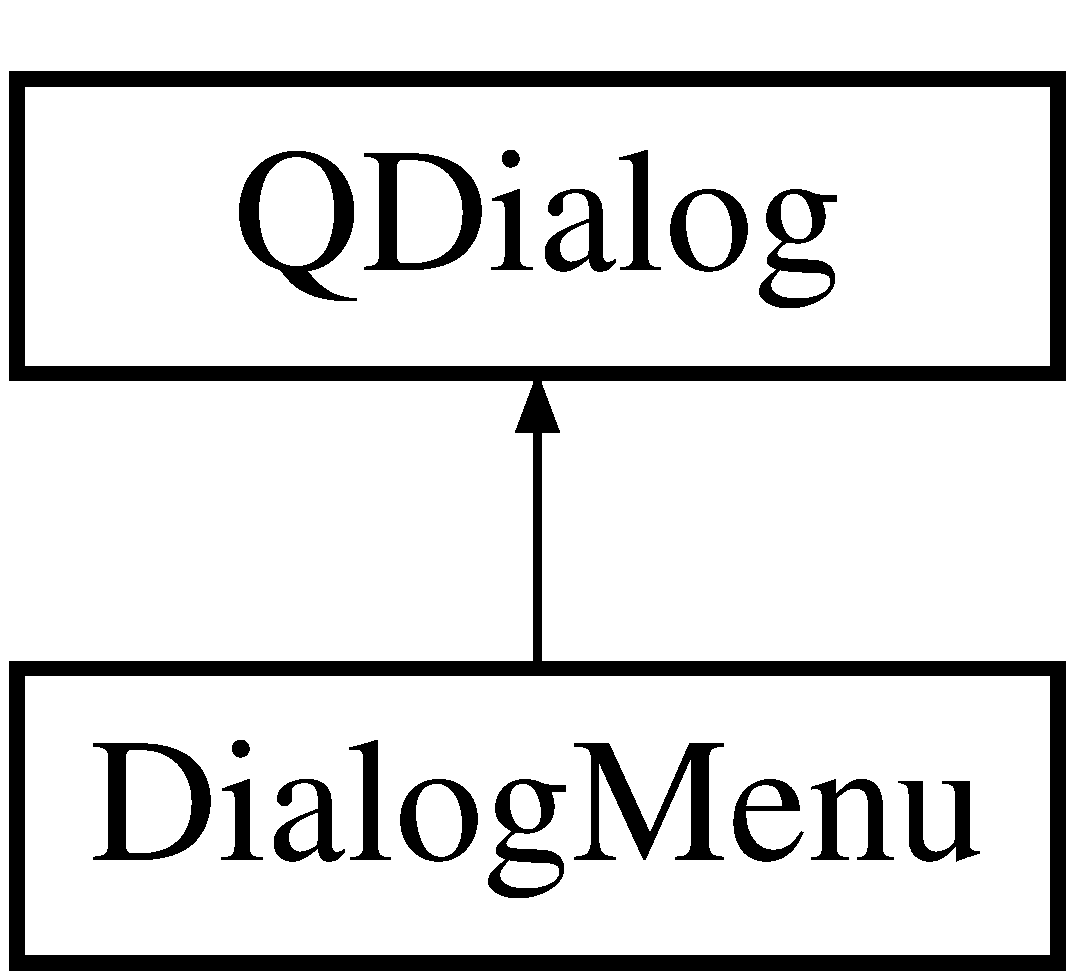
\includegraphics[height=2.000000cm]{class_dialog_menu}
\end{center}
\end{figure}
\subsection*{Public Member Functions}
\begin{DoxyCompactItemize}
\item 
\hyperlink{class_dialog_menu_a8aea7c9bd35ced81a5f6b14414e104fa}{Dialog\-Menu} (\hyperlink{class_user_data}{User\-Data} $\ast$dat, Q\-Widget $\ast$parent=0)
\begin{DoxyCompactList}\small\item\em constructor for the dialog menu window \end{DoxyCompactList}\item 
\hypertarget{class_dialog_menu_a5d6d2dbc1a3ceeefa172284963afe974}{\hyperlink{class_dialog_menu_a5d6d2dbc1a3ceeefa172284963afe974}{$\sim$\-Dialog\-Menu} ()}\label{class_dialog_menu_a5d6d2dbc1a3ceeefa172284963afe974}

\begin{DoxyCompactList}\small\item\em destructor \end{DoxyCompactList}\end{DoxyCompactItemize}
\subsection*{Private Slots}
\begin{DoxyCompactItemize}
\item 
\hypertarget{class_dialog_menu_a596866b7a1143ec8e18f74f7af1642a2}{void \hyperlink{class_dialog_menu_a596866b7a1143ec8e18f74f7af1642a2}{on\-\_\-ok\-Button\-\_\-clicked} ()}\label{class_dialog_menu_a596866b7a1143ec8e18f74f7af1642a2}

\begin{DoxyCompactList}\small\item\em callback called when the Ok button is clicked \end{DoxyCompactList}\item 
\hypertarget{class_dialog_menu_a832c6b9e32f086e1d2bf76feb2430b1b}{void \hyperlink{class_dialog_menu_a832c6b9e32f086e1d2bf76feb2430b1b}{on\-\_\-cancel\-Button\-\_\-clicked} ()}\label{class_dialog_menu_a832c6b9e32f086e1d2bf76feb2430b1b}

\begin{DoxyCompactList}\small\item\em callback called when the user click the cancel button \end{DoxyCompactList}\end{DoxyCompactItemize}
\subsection*{Private Attributes}
\begin{DoxyCompactItemize}
\item 
Ui\-::\-Dialog\-Menu $\ast$ \hyperlink{class_dialog_menu_a444aa7e99286d574d9779f728021c897}{ui}
\item 
\hyperlink{class_user_data}{User\-Data} $\ast$ \hyperlink{class_dialog_menu_af1ca62b0cbef0e0f6675a79df8b5b586}{ud}
\end{DoxyCompactItemize}


\subsection{Detailed Description}
The menu window where the user can parametrize its stabilizer inherits from Q\-Dialog. 

\subsection{Constructor \& Destructor Documentation}
\hypertarget{class_dialog_menu_a8aea7c9bd35ced81a5f6b14414e104fa}{\index{Dialog\-Menu@{Dialog\-Menu}!Dialog\-Menu@{Dialog\-Menu}}
\index{Dialog\-Menu@{Dialog\-Menu}!DialogMenu@{Dialog\-Menu}}
\subsubsection[{Dialog\-Menu}]{\setlength{\rightskip}{0pt plus 5cm}Dialog\-Menu\-::\-Dialog\-Menu (
\begin{DoxyParamCaption}
\item[{{\bf User\-Data} $\ast$}]{dat, }
\item[{Q\-Widget $\ast$}]{parent = {\ttfamily 0}}
\end{DoxyParamCaption}
)\hspace{0.3cm}{\ttfamily [explicit]}}}\label{class_dialog_menu_a8aea7c9bd35ced81a5f6b14414e104fa}


constructor for the dialog menu window 


\begin{DoxyParams}{Parameters}
{\em dat} & the user's data \\
\hline
{\em parent} & the parent window \\
\hline
\end{DoxyParams}


\subsection{Member Data Documentation}
\hypertarget{class_dialog_menu_af1ca62b0cbef0e0f6675a79df8b5b586}{\index{Dialog\-Menu@{Dialog\-Menu}!ud@{ud}}
\index{ud@{ud}!DialogMenu@{Dialog\-Menu}}
\subsubsection[{ud}]{\setlength{\rightskip}{0pt plus 5cm}{\bf User\-Data}$\ast$ Dialog\-Menu\-::ud\hspace{0.3cm}{\ttfamily [private]}}}\label{class_dialog_menu_af1ca62b0cbef0e0f6675a79df8b5b586}
pointer on the user's data \hypertarget{class_dialog_menu_a444aa7e99286d574d9779f728021c897}{\index{Dialog\-Menu@{Dialog\-Menu}!ui@{ui}}
\index{ui@{ui}!DialogMenu@{Dialog\-Menu}}
\subsubsection[{ui}]{\setlength{\rightskip}{0pt plus 5cm}Ui\-::\-Dialog\-Menu$\ast$ Dialog\-Menu\-::ui\hspace{0.3cm}{\ttfamily [private]}}}\label{class_dialog_menu_a444aa7e99286d574d9779f728021c897}
pointer on the Qt U\-I of the frame 

The documentation for this class was generated from the following files\-:\begin{DoxyCompactItemize}
\item 
dialogmenu.\-h\item 
dialogmenu.\-cpp\end{DoxyCompactItemize}

\hypertarget{class_main_window}{\section{Main\-Window Class Reference}
\label{class_main_window}\index{Main\-Window@{Main\-Window}}
}


Main window of the application, implements view and user actions inherits from Q\-Main\-Window.  




{\ttfamily \#include $<$mainwindow.\-h$>$}

Inheritance diagram for Main\-Window\-:\begin{figure}[H]
\begin{center}
\leavevmode
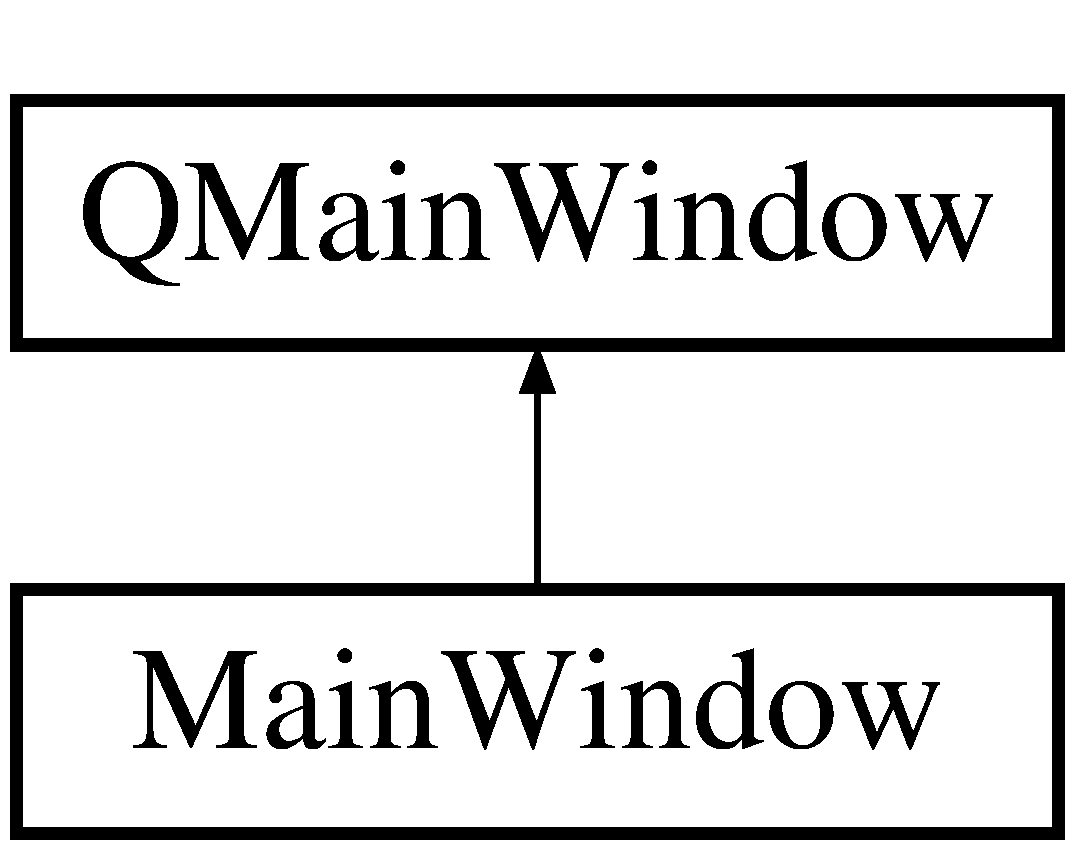
\includegraphics[height=2.000000cm]{class_main_window}
\end{center}
\end{figure}
\subsection*{Signals}
\begin{DoxyCompactItemize}
\item 
void \hyperlink{class_main_window_ad51fc5f7e60f54755507a04190f94891}{value\-To\-Send} (Q\-String val)
\begin{DoxyCompactList}\small\item\em signal emiting on user action which need to be sent to the server \end{DoxyCompactList}\end{DoxyCompactItemize}
\subsection*{Public Member Functions}
\begin{DoxyCompactItemize}
\item 
\hyperlink{class_main_window_a8b244be8b7b7db1b08de2a2acb9409db}{Main\-Window} (Q\-Widget $\ast$parent=0)
\begin{DoxyCompactList}\small\item\em main constructor \end{DoxyCompactList}\item 
\hypertarget{class_main_window_ae98d00a93bc118200eeef9f9bba1dba7}{\hyperlink{class_main_window_ae98d00a93bc118200eeef9f9bba1dba7}{$\sim$\-Main\-Window} ()}\label{class_main_window_ae98d00a93bc118200eeef9f9bba1dba7}

\begin{DoxyCompactList}\small\item\em destructor \end{DoxyCompactList}\end{DoxyCompactItemize}
\subsection*{Private Slots}
\begin{DoxyCompactItemize}
\item 
\hypertarget{class_main_window_aea3e97d7cd92a03e10cba58c85156b4c}{void \hyperlink{class_main_window_aea3e97d7cd92a03e10cba58c85156b4c}{on\-\_\-menu\-Button\-\_\-clicked} ()}\label{class_main_window_aea3e97d7cd92a03e10cba58c85156b4c}

\begin{DoxyCompactList}\small\item\em callback when user click on menu button \end{DoxyCompactList}\item 
\hypertarget{class_main_window_af06ad081f0229a31ae29a0e328e72d3b}{void \hyperlink{class_main_window_af06ad081f0229a31ae29a0e328e72d3b}{on\-\_\-x\-Plus\-Button\-\_\-clicked} ()}\label{class_main_window_af06ad081f0229a31ae29a0e328e72d3b}

\begin{DoxyCompactList}\small\item\em callback which emit a Qt signal when user click on X+ button \end{DoxyCompactList}\item 
\hypertarget{class_main_window_add37926ce0c9d9aa48a1c8e482b097e4}{void \hyperlink{class_main_window_add37926ce0c9d9aa48a1c8e482b097e4}{on\-\_\-x\-Minus\-Button\-\_\-clicked} ()}\label{class_main_window_add37926ce0c9d9aa48a1c8e482b097e4}

\begin{DoxyCompactList}\small\item\em callback which emit a Qt signal when user click on X-\/ button \end{DoxyCompactList}\item 
\hypertarget{class_main_window_a9d41c294dace3074c72ec6f8bd452fd0}{void \hyperlink{class_main_window_a9d41c294dace3074c72ec6f8bd452fd0}{on\-\_\-y\-Plus\-Button\-\_\-clicked} ()}\label{class_main_window_a9d41c294dace3074c72ec6f8bd452fd0}

\begin{DoxyCompactList}\small\item\em callback which emit a Qt signal when user click on Y+ button \end{DoxyCompactList}\item 
\hypertarget{class_main_window_ae4af2cd51d482b1009bb688ce49fe0bd}{void \hyperlink{class_main_window_ae4af2cd51d482b1009bb688ce49fe0bd}{on\-\_\-y\-Minus\-Button\-\_\-clicked} ()}\label{class_main_window_ae4af2cd51d482b1009bb688ce49fe0bd}

\begin{DoxyCompactList}\small\item\em callback which emit a Qt signal when user click on Y-\/ button \end{DoxyCompactList}\item 
\hypertarget{class_main_window_a898da68c8a89a6f3d696eb58efe8020d}{void \hyperlink{class_main_window_a898da68c8a89a6f3d696eb58efe8020d}{on\-\_\-z\-Plus\-Button\-\_\-clicked} ()}\label{class_main_window_a898da68c8a89a6f3d696eb58efe8020d}

\begin{DoxyCompactList}\small\item\em callback which emit a Qt signal when user click on Z+ button \end{DoxyCompactList}\item 
\hypertarget{class_main_window_a6c0c09ab43457ec6458127f012c0657f}{void \hyperlink{class_main_window_a6c0c09ab43457ec6458127f012c0657f}{on\-\_\-z\-Minus\-Button\-\_\-clicked} ()}\label{class_main_window_a6c0c09ab43457ec6458127f012c0657f}

\begin{DoxyCompactList}\small\item\em callback which emit a Qt signal when user click on Z-\/ button \end{DoxyCompactList}\end{DoxyCompactItemize}
\subsection*{Private Attributes}
\begin{DoxyCompactItemize}
\item 
Ui\-::\-Main\-Window $\ast$ \hyperlink{class_main_window_a35466a70ed47252a0191168126a352a5}{ui}
\item 
\hyperlink{class_user_data}{User\-Data} $\ast$ \hyperlink{class_main_window_a5ad62f9757137d68b2b49bae414c4fdd}{user}
\end{DoxyCompactItemize}


\subsection{Detailed Description}
Main window of the application, implements view and user actions inherits from Q\-Main\-Window. 

\subsection{Constructor \& Destructor Documentation}
\hypertarget{class_main_window_a8b244be8b7b7db1b08de2a2acb9409db}{\index{Main\-Window@{Main\-Window}!Main\-Window@{Main\-Window}}
\index{Main\-Window@{Main\-Window}!MainWindow@{Main\-Window}}
\subsubsection[{Main\-Window}]{\setlength{\rightskip}{0pt plus 5cm}Main\-Window\-::\-Main\-Window (
\begin{DoxyParamCaption}
\item[{Q\-Widget $\ast$}]{parent = {\ttfamily 0}}
\end{DoxyParamCaption}
)\hspace{0.3cm}{\ttfamily [explicit]}}}\label{class_main_window_a8b244be8b7b7db1b08de2a2acb9409db}


main constructor 


\begin{DoxyParams}{Parameters}
{\em parent} & the parent creating the window (no parent in our caseà \\
\hline
\end{DoxyParams}


\subsection{Member Function Documentation}
\hypertarget{class_main_window_ad51fc5f7e60f54755507a04190f94891}{\index{Main\-Window@{Main\-Window}!value\-To\-Send@{value\-To\-Send}}
\index{value\-To\-Send@{value\-To\-Send}!MainWindow@{Main\-Window}}
\subsubsection[{value\-To\-Send}]{\setlength{\rightskip}{0pt plus 5cm}void Main\-Window\-::value\-To\-Send (
\begin{DoxyParamCaption}
\item[{Q\-String}]{val}
\end{DoxyParamCaption}
)\hspace{0.3cm}{\ttfamily [signal]}}}\label{class_main_window_ad51fc5f7e60f54755507a04190f94891}


signal emiting on user action which need to be sent to the server 


\begin{DoxyParams}{Parameters}
{\em val} & the string to emit \\
\hline
\end{DoxyParams}


\subsection{Member Data Documentation}
\hypertarget{class_main_window_a35466a70ed47252a0191168126a352a5}{\index{Main\-Window@{Main\-Window}!ui@{ui}}
\index{ui@{ui}!MainWindow@{Main\-Window}}
\subsubsection[{ui}]{\setlength{\rightskip}{0pt plus 5cm}Ui\-::\-Main\-Window$\ast$ Main\-Window\-::ui\hspace{0.3cm}{\ttfamily [private]}}}\label{class_main_window_a35466a70ed47252a0191168126a352a5}
pointer on the Qt U\-I \hypertarget{class_main_window_a5ad62f9757137d68b2b49bae414c4fdd}{\index{Main\-Window@{Main\-Window}!user@{user}}
\index{user@{user}!MainWindow@{Main\-Window}}
\subsubsection[{user}]{\setlength{\rightskip}{0pt plus 5cm}{\bf User\-Data}$\ast$ Main\-Window\-::user\hspace{0.3cm}{\ttfamily [private]}}}\label{class_main_window_a5ad62f9757137d68b2b49bae414c4fdd}
pointer on the user's data 

The documentation for this class was generated from the following files\-:\begin{DoxyCompactItemize}
\item 
mainwindow.\-h\item 
mainwindow.\-cpp\end{DoxyCompactItemize}

\hypertarget{class_thread_receiving}{\section{Thread\-Receiving Class Reference}
\label{class_thread_receiving}\index{Thread\-Receiving@{Thread\-Receiving}}
}


thread establishing connections and receives data from the server  




{\ttfamily \#include $<$serverthread.\-h$>$}

Inheritance diagram for Thread\-Receiving\-:\begin{figure}[H]
\begin{center}
\leavevmode
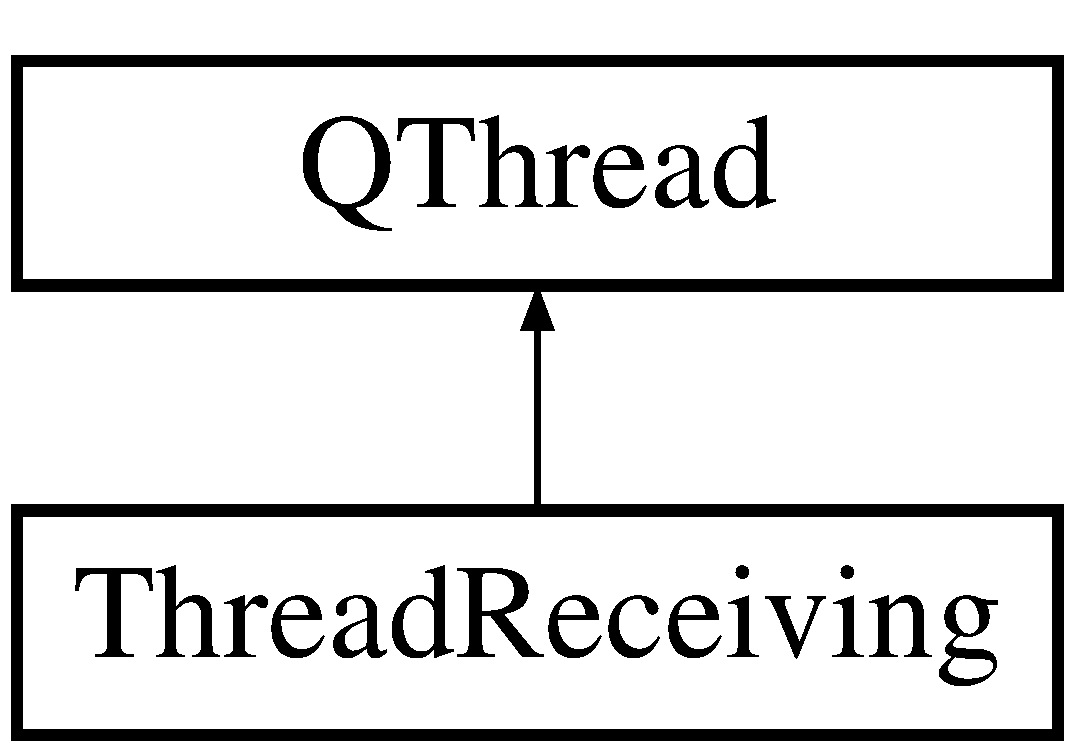
\includegraphics[height=2.000000cm]{class_thread_receiving}
\end{center}
\end{figure}
\subsection*{Public Member Functions}
\begin{DoxyCompactItemize}
\item 
\hypertarget{class_thread_receiving_a027544891898af6371f5b113e55ef261}{\hyperlink{class_thread_receiving_a027544891898af6371f5b113e55ef261}{Thread\-Receiving} ()}\label{class_thread_receiving_a027544891898af6371f5b113e55ef261}

\begin{DoxyCompactList}\small\item\em constructor initialize I\-P and port \end{DoxyCompactList}\end{DoxyCompactItemize}
\subsection*{Private Member Functions}
\begin{DoxyCompactItemize}
\item 
\hypertarget{class_thread_receiving_adce995539c66e751f0e6028aac9a2873}{void \hyperlink{class_thread_receiving_adce995539c66e751f0e6028aac9a2873}{run} ()}\label{class_thread_receiving_adce995539c66e751f0e6028aac9a2873}

\begin{DoxyCompactList}\small\item\em method call when the thread starts \end{DoxyCompactList}\end{DoxyCompactItemize}
\subsection*{Private Attributes}
\begin{DoxyCompactItemize}
\item 
Q\-String \hyperlink{class_thread_receiving_a8f4461638c9b0441e58b72ab427306ef}{server\-I\-P}
\item 
int \hyperlink{class_thread_receiving_ae76ea6b3c01277dad2ffa27d8a3feae4}{port\-Read}
\end{DoxyCompactItemize}


\subsection{Detailed Description}
thread establishing connections and receives data from the server 

\subsection{Member Data Documentation}
\hypertarget{class_thread_receiving_ae76ea6b3c01277dad2ffa27d8a3feae4}{\index{Thread\-Receiving@{Thread\-Receiving}!port\-Read@{port\-Read}}
\index{port\-Read@{port\-Read}!ThreadReceiving@{Thread\-Receiving}}
\subsubsection[{port\-Read}]{\setlength{\rightskip}{0pt plus 5cm}int Thread\-Receiving\-::port\-Read\hspace{0.3cm}{\ttfamily [private]}}}\label{class_thread_receiving_ae76ea6b3c01277dad2ffa27d8a3feae4}
port used for connection \hypertarget{class_thread_receiving_a8f4461638c9b0441e58b72ab427306ef}{\index{Thread\-Receiving@{Thread\-Receiving}!server\-I\-P@{server\-I\-P}}
\index{server\-I\-P@{server\-I\-P}!ThreadReceiving@{Thread\-Receiving}}
\subsubsection[{server\-I\-P}]{\setlength{\rightskip}{0pt plus 5cm}Q\-String Thread\-Receiving\-::server\-I\-P\hspace{0.3cm}{\ttfamily [private]}}}\label{class_thread_receiving_a8f4461638c9b0441e58b72ab427306ef}
the server I\-P 

The documentation for this class was generated from the following files\-:\begin{DoxyCompactItemize}
\item 
serverthread.\-h\item 
serverthread.\-cpp\end{DoxyCompactItemize}

\hypertarget{class_thread_sending}{\section{Thread\-Sending Class Reference}
\label{class_thread_sending}\index{Thread\-Sending@{Thread\-Sending}}
}


thread establishing connection with server and sends data to the server inherits from Q\-Thread  




{\ttfamily \#include $<$serverthread.\-h$>$}

Inheritance diagram for Thread\-Sending\-:\begin{figure}[H]
\begin{center}
\leavevmode
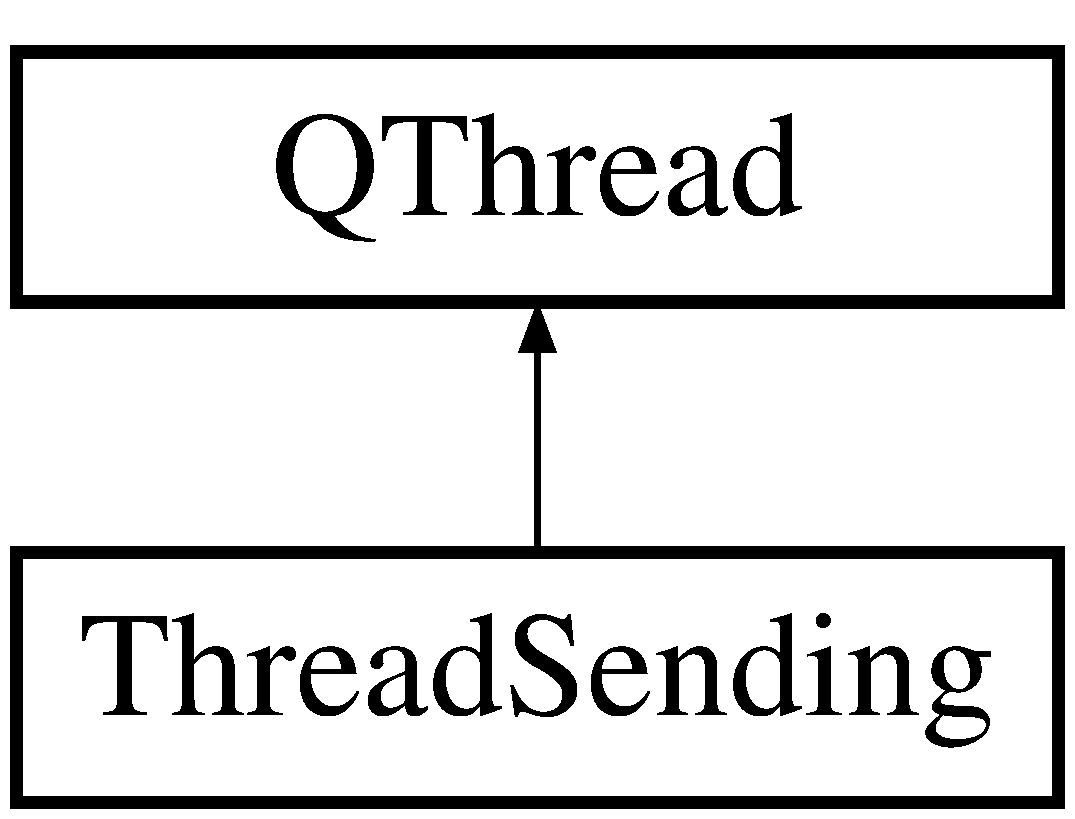
\includegraphics[height=2.000000cm]{class_thread_sending}
\end{center}
\end{figure}
\subsection*{Public Slots}
\begin{DoxyCompactItemize}
\item 
void \hyperlink{class_thread_sending_aae57341ed5f031338c6ba10f35d277c5}{add\-Value\-To\-List} (Q\-String val)
\begin{DoxyCompactList}\small\item\em the slot which receives signals sent by \hyperlink{class_main_window}{Main\-Window} \end{DoxyCompactList}\end{DoxyCompactItemize}
\subsection*{Public Member Functions}
\begin{DoxyCompactItemize}
\item 
\hypertarget{class_thread_sending_abdd5e874ce261b64bde9066e4369904f}{\hyperlink{class_thread_sending_abdd5e874ce261b64bde9066e4369904f}{Thread\-Sending} ()}\label{class_thread_sending_abdd5e874ce261b64bde9066e4369904f}

\begin{DoxyCompactList}\small\item\em constructor, initiliaze I\-P and port \end{DoxyCompactList}\end{DoxyCompactItemize}
\subsection*{Private Member Functions}
\begin{DoxyCompactItemize}
\item 
\hypertarget{class_thread_sending_a5f3612a36c9fb8a1861665aeb2c3f60b}{void \hyperlink{class_thread_sending_a5f3612a36c9fb8a1861665aeb2c3f60b}{run} ()}\label{class_thread_sending_a5f3612a36c9fb8a1861665aeb2c3f60b}

\begin{DoxyCompactList}\small\item\em method call when the thread starts \end{DoxyCompactList}\end{DoxyCompactItemize}
\subsection*{Private Attributes}
\begin{DoxyCompactItemize}
\item 
Q\-String \hyperlink{class_thread_sending_aeb557d91ac550a8efce1d43e130392f8}{server\-I\-P}
\item 
int \hyperlink{class_thread_sending_aa97703aeda03c6a18b2f300558ba5ae0}{port\-Write}
\item 
Q\-List$<$ Q\-String $>$ \hyperlink{class_thread_sending_a381edbf0d9460a47a9a75a27c3918ae6}{to\-Send}
\item 
Q\-Mutex \hyperlink{class_thread_sending_acf56dd5ae4ee3ac319e93307c6ef74ea}{mutex}
\end{DoxyCompactItemize}


\subsection{Detailed Description}
thread establishing connection with server and sends data to the server inherits from Q\-Thread 

\subsection{Member Function Documentation}
\hypertarget{class_thread_sending_aae57341ed5f031338c6ba10f35d277c5}{\index{Thread\-Sending@{Thread\-Sending}!add\-Value\-To\-List@{add\-Value\-To\-List}}
\index{add\-Value\-To\-List@{add\-Value\-To\-List}!ThreadSending@{Thread\-Sending}}
\subsubsection[{add\-Value\-To\-List}]{\setlength{\rightskip}{0pt plus 5cm}void Thread\-Sending\-::add\-Value\-To\-List (
\begin{DoxyParamCaption}
\item[{Q\-String}]{val}
\end{DoxyParamCaption}
)\hspace{0.3cm}{\ttfamily [slot]}}}\label{class_thread_sending_aae57341ed5f031338c6ba10f35d277c5}


the slot which receives signals sent by \hyperlink{class_main_window}{Main\-Window} 


\begin{DoxyParams}{Parameters}
{\em val} & the string emitted \\
\hline
\end{DoxyParams}


\subsection{Member Data Documentation}
\hypertarget{class_thread_sending_acf56dd5ae4ee3ac319e93307c6ef74ea}{\index{Thread\-Sending@{Thread\-Sending}!mutex@{mutex}}
\index{mutex@{mutex}!ThreadSending@{Thread\-Sending}}
\subsubsection[{mutex}]{\setlength{\rightskip}{0pt plus 5cm}Q\-Mutex Thread\-Sending\-::mutex\hspace{0.3cm}{\ttfamily [private]}}}\label{class_thread_sending_acf56dd5ae4ee3ac319e93307c6ef74ea}
mutex used to avoid concurrent access on list \hypertarget{class_thread_sending_aa97703aeda03c6a18b2f300558ba5ae0}{\index{Thread\-Sending@{Thread\-Sending}!port\-Write@{port\-Write}}
\index{port\-Write@{port\-Write}!ThreadSending@{Thread\-Sending}}
\subsubsection[{port\-Write}]{\setlength{\rightskip}{0pt plus 5cm}int Thread\-Sending\-::port\-Write\hspace{0.3cm}{\ttfamily [private]}}}\label{class_thread_sending_aa97703aeda03c6a18b2f300558ba5ae0}
the port where it connects \hypertarget{class_thread_sending_aeb557d91ac550a8efce1d43e130392f8}{\index{Thread\-Sending@{Thread\-Sending}!server\-I\-P@{server\-I\-P}}
\index{server\-I\-P@{server\-I\-P}!ThreadSending@{Thread\-Sending}}
\subsubsection[{server\-I\-P}]{\setlength{\rightskip}{0pt plus 5cm}Q\-String Thread\-Sending\-::server\-I\-P\hspace{0.3cm}{\ttfamily [private]}}}\label{class_thread_sending_aeb557d91ac550a8efce1d43e130392f8}
the I\-P of the server \hypertarget{class_thread_sending_a381edbf0d9460a47a9a75a27c3918ae6}{\index{Thread\-Sending@{Thread\-Sending}!to\-Send@{to\-Send}}
\index{to\-Send@{to\-Send}!ThreadSending@{Thread\-Sending}}
\subsubsection[{to\-Send}]{\setlength{\rightskip}{0pt plus 5cm}Q\-List$<$Q\-String$>$ Thread\-Sending\-::to\-Send\hspace{0.3cm}{\ttfamily [private]}}}\label{class_thread_sending_a381edbf0d9460a47a9a75a27c3918ae6}
list of data to send 

The documentation for this class was generated from the following files\-:\begin{DoxyCompactItemize}
\item 
serverthread.\-h\item 
serverthread.\-cpp\end{DoxyCompactItemize}

\hypertarget{class_user_data}{\section{User\-Data Class Reference}
\label{class_user_data}\index{User\-Data@{User\-Data}}
}


represents the user data(the offset he has chosen for his stabilizer)  




{\ttfamily \#include $<$userdata.\-h$>$}

\subsection*{Public Member Functions}
\begin{DoxyCompactItemize}
\item 
\hypertarget{class_user_data_a1d4f7b61ec5dd67bbd4e03efd4f85ce8}{\hyperlink{class_user_data_a1d4f7b61ec5dd67bbd4e03efd4f85ce8}{User\-Data} ()}\label{class_user_data_a1d4f7b61ec5dd67bbd4e03efd4f85ce8}

\begin{DoxyCompactList}\small\item\em main constructor \end{DoxyCompactList}\item 
int \hyperlink{class_user_data_aab9e0256d899b0ebd42f6ce5ab943b3e}{get\-X} ()
\begin{DoxyCompactList}\small\item\em getter X \end{DoxyCompactList}\item 
int \hyperlink{class_user_data_a526578c6937e9d36eb375621418ddfbc}{get\-Y} ()
\begin{DoxyCompactList}\small\item\em getter Y \end{DoxyCompactList}\item 
int \hyperlink{class_user_data_af1c783c40df183b19d1c1bf6779d9232}{get\-Z} ()
\begin{DoxyCompactList}\small\item\em getter Z \end{DoxyCompactList}\item 
void \hyperlink{class_user_data_ae8f570275ee8cc51fb86657a77730fab}{set\-X} (int)
\begin{DoxyCompactList}\small\item\em setter x \end{DoxyCompactList}\item 
void \hyperlink{class_user_data_a263a40e7bf596509b02954c0bb017f5f}{set\-Y} (int)
\begin{DoxyCompactList}\small\item\em setter y \end{DoxyCompactList}\item 
void \hyperlink{class_user_data_a73d14105631aced4993ce7d3ec5bf3e5}{set\-Z} (int)
\begin{DoxyCompactList}\small\item\em setter z \end{DoxyCompactList}\end{DoxyCompactItemize}
\subsection*{Private Attributes}
\begin{DoxyCompactItemize}
\item 
int \hyperlink{class_user_data_a92294b82200b514e4cf5ae95209a9506}{x}
\item 
int \hyperlink{class_user_data_afa979b1e92775250f576874cab5d9dee}{y}
\item 
int \hyperlink{class_user_data_a724828d778bda060073712c5d87ae7c4}{z}
\end{DoxyCompactItemize}


\subsection{Detailed Description}
represents the user data(the offset he has chosen for his stabilizer) 

\subsection{Member Function Documentation}
\hypertarget{class_user_data_aab9e0256d899b0ebd42f6ce5ab943b3e}{\index{User\-Data@{User\-Data}!get\-X@{get\-X}}
\index{get\-X@{get\-X}!UserData@{User\-Data}}
\subsubsection[{get\-X}]{\setlength{\rightskip}{0pt plus 5cm}int User\-Data\-::get\-X (
\begin{DoxyParamCaption}
{}
\end{DoxyParamCaption}
)}}\label{class_user_data_aab9e0256d899b0ebd42f6ce5ab943b3e}


getter X 

\begin{DoxyReturn}{Returns}
int x 
\end{DoxyReturn}
\hypertarget{class_user_data_a526578c6937e9d36eb375621418ddfbc}{\index{User\-Data@{User\-Data}!get\-Y@{get\-Y}}
\index{get\-Y@{get\-Y}!UserData@{User\-Data}}
\subsubsection[{get\-Y}]{\setlength{\rightskip}{0pt plus 5cm}int User\-Data\-::get\-Y (
\begin{DoxyParamCaption}
{}
\end{DoxyParamCaption}
)}}\label{class_user_data_a526578c6937e9d36eb375621418ddfbc}


getter Y 

\begin{DoxyReturn}{Returns}
int y 
\end{DoxyReturn}
\hypertarget{class_user_data_af1c783c40df183b19d1c1bf6779d9232}{\index{User\-Data@{User\-Data}!get\-Z@{get\-Z}}
\index{get\-Z@{get\-Z}!UserData@{User\-Data}}
\subsubsection[{get\-Z}]{\setlength{\rightskip}{0pt plus 5cm}int User\-Data\-::get\-Z (
\begin{DoxyParamCaption}
{}
\end{DoxyParamCaption}
)}}\label{class_user_data_af1c783c40df183b19d1c1bf6779d9232}


getter Z 

\begin{DoxyReturn}{Returns}
int e 
\end{DoxyReturn}
\hypertarget{class_user_data_ae8f570275ee8cc51fb86657a77730fab}{\index{User\-Data@{User\-Data}!set\-X@{set\-X}}
\index{set\-X@{set\-X}!UserData@{User\-Data}}
\subsubsection[{set\-X}]{\setlength{\rightskip}{0pt plus 5cm}void User\-Data\-::set\-X (
\begin{DoxyParamCaption}
\item[{int}]{val}
\end{DoxyParamCaption}
)}}\label{class_user_data_ae8f570275ee8cc51fb86657a77730fab}


setter x 


\begin{DoxyParams}{Parameters}
{\em int} & new value of x \\
\hline
\end{DoxyParams}
\hypertarget{class_user_data_a263a40e7bf596509b02954c0bb017f5f}{\index{User\-Data@{User\-Data}!set\-Y@{set\-Y}}
\index{set\-Y@{set\-Y}!UserData@{User\-Data}}
\subsubsection[{set\-Y}]{\setlength{\rightskip}{0pt plus 5cm}void User\-Data\-::set\-Y (
\begin{DoxyParamCaption}
\item[{int}]{val}
\end{DoxyParamCaption}
)}}\label{class_user_data_a263a40e7bf596509b02954c0bb017f5f}


setter y 


\begin{DoxyParams}{Parameters}
{\em int} & new value of y \\
\hline
\end{DoxyParams}
\hypertarget{class_user_data_a73d14105631aced4993ce7d3ec5bf3e5}{\index{User\-Data@{User\-Data}!set\-Z@{set\-Z}}
\index{set\-Z@{set\-Z}!UserData@{User\-Data}}
\subsubsection[{set\-Z}]{\setlength{\rightskip}{0pt plus 5cm}void User\-Data\-::set\-Z (
\begin{DoxyParamCaption}
\item[{int}]{val}
\end{DoxyParamCaption}
)}}\label{class_user_data_a73d14105631aced4993ce7d3ec5bf3e5}


setter z 


\begin{DoxyParams}{Parameters}
{\em int} & new value of z \\
\hline
\end{DoxyParams}


\subsection{Member Data Documentation}
\hypertarget{class_user_data_a92294b82200b514e4cf5ae95209a9506}{\index{User\-Data@{User\-Data}!x@{x}}
\index{x@{x}!UserData@{User\-Data}}
\subsubsection[{x}]{\setlength{\rightskip}{0pt plus 5cm}int User\-Data\-::x\hspace{0.3cm}{\ttfamily [private]}}}\label{class_user_data_a92294b82200b514e4cf5ae95209a9506}
offstet in degree on X axis \hypertarget{class_user_data_afa979b1e92775250f576874cab5d9dee}{\index{User\-Data@{User\-Data}!y@{y}}
\index{y@{y}!UserData@{User\-Data}}
\subsubsection[{y}]{\setlength{\rightskip}{0pt plus 5cm}int User\-Data\-::y\hspace{0.3cm}{\ttfamily [private]}}}\label{class_user_data_afa979b1e92775250f576874cab5d9dee}
offstet in degree on Y axis \hypertarget{class_user_data_a724828d778bda060073712c5d87ae7c4}{\index{User\-Data@{User\-Data}!z@{z}}
\index{z@{z}!UserData@{User\-Data}}
\subsubsection[{z}]{\setlength{\rightskip}{0pt plus 5cm}int User\-Data\-::z\hspace{0.3cm}{\ttfamily [private]}}}\label{class_user_data_a724828d778bda060073712c5d87ae7c4}
offstet in degree on Z axis 

The documentation for this class was generated from the following files\-:\begin{DoxyCompactItemize}
\item 
userdata.\-h\item 
userdata.\-cpp\end{DoxyCompactItemize}

%--- End generated contents ---

% Index
\newpage
\phantomsection
\addcontentsline{toc}{chapter}{Index}
\printindex

\end{document}
